\documentclass[aspectratio=169]{beamer}

\usepackage[T1]{fontenc}
\usepackage{amsmath}
\usepackage{amssymb}
\usepackage{graphicx}
\usepackage{tikz}
\usetikzlibrary{shapes.geometric, arrows.meta, positioning}

\definecolor{coolpurple}{HTML}{7f65a0}
\definecolor{lightpurple}{HTML}{ede8f5}
\definecolor{darktext}{HTML}{1a1a2e}
\definecolor{highlightpurple}{HTML}{5a3e82}

\setbeamercolor{normal text}{fg=darktext, bg=white}
\setbeamercolor{structure}{fg=coolpurple}
\setbeamercolor{frametitle}{fg=white, bg=coolpurple}
\setbeamercolor{title}{fg=white, bg=coolpurple}
\setbeamercolor{subtitle}{fg=white}
\setbeamercolor{date}{fg=coolpurple}
\setbeamercolor{author}{fg=coolpurple}
\setbeamercolor{item}{fg=coolpurple}
\setbeamercolor{subitem}{fg=coolpurple!70!black}
\setbeamercolor{block title}{bg=coolpurple, fg=white}
\setbeamercolor{block body}{bg=lightpurple, fg=darktext}
\setbeamercolor{alerted text}{fg=highlightpurple}

\setbeamertemplate{itemize item}{\color{coolpurple}$\blacktriangleright$}
\setbeamertemplate{itemize subitem}{\color{coolpurple!70}$\bullet$}
\setbeamertemplate{navigation symbols}{}
\setbeamertemplate{footline}{%
	\hfill\insertframenumber\,/\,\inserttotalframenumber\hspace{1em}\vspace{0.5em}
}

\newcommand{\hl}[1]{\textcolor{coolpurple}{\textbf{#1}}}
\newcommand{\R}{\mathbb{R}}

\title{EngageNet}
\subtitle{Progress Update - September 23, 2026}
\author{Lado Turmanidze}
\institute{\small{Supervisors: Dr. Philipp M\"{u}ller \& Beso Mikaberidze}}
\date{September 23, 2026}

\begin{document}

	\begin{frame}
		\titlepage
	\end{frame}

	\begin{frame}{The Short Version}
		\begin{block}{What happened since the last meeting}
			The model was built, it trained, and it produced numbers - but the numbers were bad.
			\vspace{0.4em}

			I went looking for \emph{why}, and found six problems. Two of them are not opinions:
			they are arithmetic. The model literally could not do what we designed it to do.
		\end{block}
		\vspace{0.5em}
		\begin{center}
			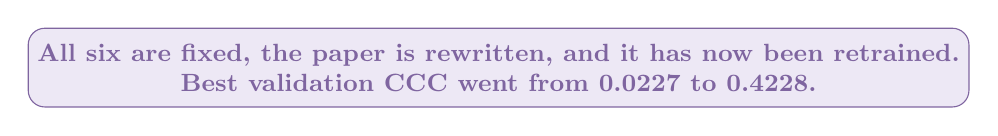
\begin{tikzpicture}
				\node[draw=coolpurple, fill=lightpurple, rounded corners=6pt,
				minimum width=11cm, minimum height=1.0cm, align=center,
				font=\small\bfseries, text=coolpurple] {
					All six are fixed, the paper is rewritten, and it has now been retrained.\\
					Best validation CCC went from \textbf{0.0227} to \textbf{0.4228}.
				};
			\end{tikzpicture}
		\end{center}
	\end{frame}

	\begin{frame}{Today's Agenda}
		\begin{enumerate}
			\item \textbf{Recap} - what the task is, what the model does
			\item \textbf{Where we stood} - the numbers that started this
			\item \textbf{The map} - a small theorem telling us where to look
			\item \textbf{Problem 1} - the model had no memory
			\item \textbf{Problem 2} - the modalities never talked to each other
			\item \textbf{Problem 3} - we predicted the wrong thing
			\item \textbf{Problem 4} - the loss function had three bugs
			\item \textbf{Results} - what the retrained model actually does
			\item \textbf{Since August} - checking our own numbers, and a method that never ran
			\item \textbf{What we fixed, and what is next}
		\end{enumerate}
	\end{frame}

	% ============================== PART 0: RECAP ==============================

	\begin{frame}{\textsc{Part 0:} What Is The Task?}
		\begin{columns}[onlytextwidth]
			\begin{column}{0.52\textwidth}
				\begin{block}{The setup}
					\small
					Two people talk over a video link. One is the \hl{expert} (explains something
					they love), one is the \hl{novice} (listens, asks questions).
					\vspace{0.3em}

					Human annotators watch the recording and move a slider to say
					\emph{how engaged is this person, right now}.
				\end{block}
			\end{column}
			\begin{column}{0.44\textwidth}
				\begin{block}{Our job}
					\small
					For \textbf{every frame} of video, and for \textbf{each of the two people},
					predict that slider value.
					$$ y_t \in [0,1], \qquad 25 \text{ frames per second} $$
				\end{block}
			\end{column}
		\end{columns}
		\vspace{0.5em}
		\centering\small
		A 10-minute session is $\sim$15{,}000 numbers per person. We predict all of them.
	\end{frame}

	\begin{frame}{Recap - The Data We Get}
		\begin{columns}[onlytextwidth]
			\begin{column}{0.48\textwidth}
				\begin{block}{Four feature types $\mathcal{F}$}
					\small
					\begin{itemize}
						\item eGeMAPS v2 - acoustic descriptors
						\item W2v-BERT 2.0 - learned speech embedding
						\item OpenFace2 - facial action units
						\item OpenPose - body keypoints
					\end{itemize}
				\end{block}
			\end{column}
			\begin{column}{0.48\textwidth}
				\begin{block}{Two roles $\mathcal{R}$}
					\small
					Separate camera and microphone per person, so \textbf{every feature type
					arrives twice}:
					$$ M = |\mathcal{F}| \times |\mathcal{R}| = 4 \times 2 = 8 $$
					8 parallel streams into the network.
				\end{block}
			\end{column}
		\end{columns}
		\vspace{0.5em}
		\begin{center}
			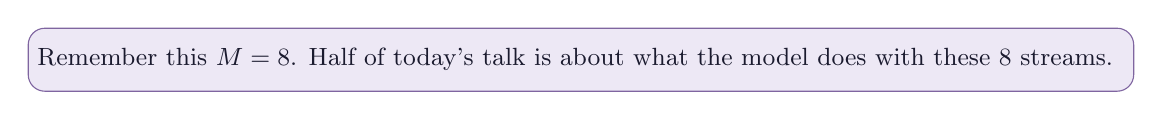
\begin{tikzpicture}
				\node[draw=coolpurple, fill=lightpurple, rounded corners=6pt,
				minimum width=11cm, minimum height=0.8cm, align=center,
				font=\small, text=darktext] {
					Remember this $M = 8$. Half of today's talk is about what the model does
					with these 8 streams.
				};
			\end{tikzpicture}
		\end{center}
	\end{frame}

	\begin{frame}{Recap - Architecture}
		\centering
		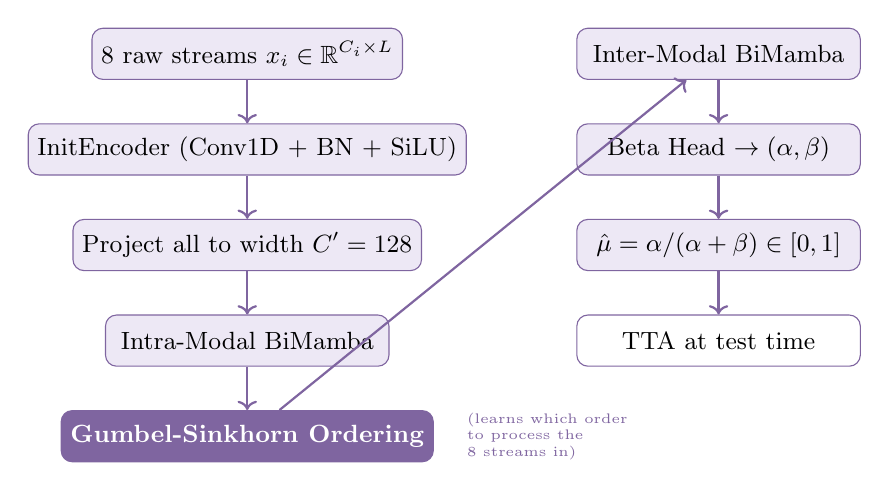
\begin{tikzpicture}[
			node distance=0.55cm,
			font=\small,
			box/.style={draw=coolpurple, fill=lightpurple, rounded corners,
				minimum width=3.6cm, minimum height=0.65cm, align=center}
			]

			\node[box] (input) {8 raw streams $x_i \in \R^{C_i \times L}$};
			\node[box, below=of input] (enc) {InitEncoder (Conv1D + BN + SiLU)};
			\node[box, below=of enc] (proj) {Project all to width $C'=128$};
			\node[box, below=of proj] (intra) {Intra-Modal BiMamba};
			\node[box, below=of intra, fill=coolpurple, text=white, font=\small\bfseries] (gs) {Gumbel-Sinkhorn Ordering};

			\node[box, right=2.2cm of input] (inter) {Inter-Modal BiMamba};
			\node[box, below=of inter] (beta) {Beta Head $\to (\alpha, \beta)$};
			\node[box, below=of beta] (out) {$\hat{\mu} = \alpha/(\alpha+\beta) \in [0,1]$};
			\node[box, below=of out, fill=white] (tta) {TTA at test time};

			\foreach \a/\b in {input/enc, enc/proj, proj/intra, intra/gs, gs/inter, inter/beta, beta/out, out/tta} {
				\draw[->, thick, coolpurple] (\a) -- (\b);
			}

			\node[right=0.3cm of gs, text=coolpurple, font=\tiny, align=left]
			{(learns which order \\ to process the \\ 8 streams in)};

		\end{tikzpicture}
	\end{frame}

	\begin{frame}{Recap - What A State-Space Model Actually Does}
		\begin{block}{One line of maths, and it is the whole idea}
			$$ \xi_t = \bar{A}\,\xi_{t-1} + \bar{B}_t u_t $$
			\small
			$\xi_t$ is the model's \hl{memory} at step $t$. Each step it keeps a fraction
			$\bar{A}$ of what it remembered, and adds in the new input $u_t$.
		\end{block}
		\vspace{0.3em}
		\begin{columns}[onlytextwidth]
			\begin{column}{0.48\textwidth}
				\begin{block}{Why this shape}
					\small
					$\bar{A} \in (0,1)$, so old information fades smoothly instead of
					blowing up. Nice and stable.
				\end{block}
			\end{column}
			\begin{column}{0.48\textwidth}
				\begin{block}{Why it is fast}
					\small
					Looks sequential, but the update is \emph{affine}, so we can compute all
					$L$ steps with an associative scan in $O(\log L)$ depth instead of $O(L)$.
				\end{block}
			\end{column}
		\end{columns}
		\vspace{0.4em}
		\centering\small
		\hl{Keep $\bar{A}$ in mind.} Problems 1 and 2 are both about this one number.
	\end{frame}

	\begin{frame}{Recap - Why Beta Instead Of A Plain Number}
		\begin{columns}[onlytextwidth]
			\begin{column}{0.50\textwidth}
				\begin{block}{The model outputs a distribution}
					\small
					Not one number, but two: $(\alpha, \beta)$, defining
					$$ p(y \mid x) = \mathrm{Beta}(\alpha, \beta), \quad y \in [0,1] $$
					Prediction is the mean $\hat{\mu} = \frac{\alpha}{\alpha+\beta}$.
				\end{block}
			\end{column}
			\begin{column}{0.46\textwidth}
				\begin{block}{Why bother}
					\small
					The \emph{spread} tells us how sure the model is:
					$$ \mathrm{Var}[y] = \frac{\alpha\beta}{(\alpha+\beta)^2(\alpha+\beta+1)} $$
					Test-time adaptation uses this to pick which unlabelled frames are safe
					to learn from.
				\end{block}
			\end{column}
		\end{columns}
		\vspace{0.5em}
		\centering\small
		Beta lives on $[0,1]$ - exactly the range of engagement. A Gaussian would put
		probability on $-0.3$ and $1.4$, which are not things.
	\end{frame}

	% ============================== PART 1: THE NUMBERS ==============================

	\begin{frame}{\textsc{Part 1:} Where We Stood}
		\begin{columns}[onlytextwidth]
			\begin{column}{0.48\textwidth}
				\begin{alertblock}{What training gave us}
					\small
					\begin{itemize}
						\item Best validation CCC: \hl{0.0227}
						\item Reached at epoch 2, then flat
						\item Correlation $\rho \approx 0.229$
						\item 7.2M parameters
					\end{itemize}
				\end{alertblock}
			\end{column}
			\begin{column}{0.48\textwidth}
				\begin{block}{What the leaderboard looks like}
					\small
					\begin{tabular}{lr}
						Official baseline & 0.400 \\
						2025 winner & 0.699 \\
						\hline
						\textbf{Us} & \textbf{0.02} \\
					\end{tabular}
				\end{block}
			\end{column}
		\end{columns}
		\vspace{0.6em}
		\begin{center}
			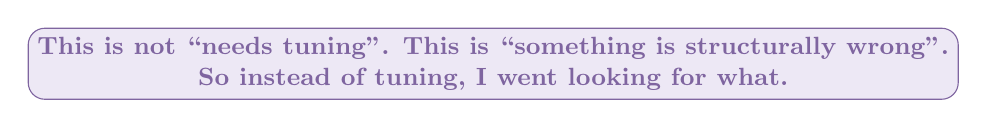
\begin{tikzpicture}
				\node[draw=coolpurple, fill=lightpurple, rounded corners=6pt,
				minimum width=11cm, minimum height=0.9cm, align=center,
				font=\small\bfseries, text=coolpurple] {
					This is not ``needs tuning''. This is ``something is structurally wrong''.\\
					So instead of tuning, I went looking for what.
				};
			\end{tikzpicture}
		\end{center}
	\end{frame}

	% ============================== PART 2: THE MAP ==============================

	\begin{frame}{\textsc{Part 2:} A Small Theorem That Told Us Where To Look}
		\begin{block}{Split CCC into two factors}
			\small
			Let $\varphi = \sigma_{\hat{y}}/\sigma_y$ (are the predictions as spread out as the truth?)
			and $\omega = (\mu_{\hat{y}}-\mu_y)/\sqrt{\sigma_{\hat{y}}\sigma_y}$ (are they centred right?). Then
			$$ \text{CCC} = \rho \cdot C_b, \qquad C_b = \frac{2}{\varphi + \varphi^{-1} + \omega^2} $$
		\end{block}
		\begin{block}{Proposition}
			\small
			$\text{CCC} \le \rho$, with equality only when $\sigma_{\hat{y}} = \sigma_y$ and $\mu_{\hat{y}} = \mu_y$.
			\vspace{0.3em}

			\emph{Proof.} $\varphi + \varphi^{-1} \ge 2$ for any $\varphi > 0$ (AM-GM), and $\omega^2 \ge 0$.
			So the denominator of $C_b$ is at least $2$, giving $C_b \le 1$. $\square$
		\end{block}
		\vspace{0.3em}
		\centering\small
		\hl{Translation:} correlation is a hard ceiling. Rescaling the output can never beat it.
	\end{frame}

	\begin{frame}{What The Theorem Told Us}
		\begin{columns}[onlytextwidth]
			\begin{column}{0.48\textwidth}
				\begin{alertblock}{Where we were (5 weeks ago)}
					\small
					$$ \rho = 0.229, \qquad \text{CCC} = 0.21 $$
					$$ \implies C_b = \frac{0.21}{0.229} \approx 0.92 $$
					Already $92\%$ calibrated - so rescaling the output could buy at most
					$0.229 - 0.21 = 0.02$.
				\end{alertblock}
			\end{column}
			\begin{column}{0.48\textwidth}
				\begin{block}{Where we are now (NoXi, epoch 16)}
					\small
					$$ \rho = 0.7951, \qquad \text{CCC} = 0.7942 $$
					$$ \implies C_b = \frac{0.7942}{0.7951} = \hl{0.9989} $$
					Calibration is now essentially perfect. The gap the theorem said was
					closable, we closed.
				\end{block}
			\end{column}
		\end{columns}
	\end{frame}

	% ============================== PROBLEM 1 ==============================

	\begin{frame}{\textsc{Problem 1:} The Model Had A Goldfish Memory}
		\begin{block}{How long does an SSM remember?}
			\small
			Stop feeding it input. Then $\xi_{t_0+k} = \bar{A}^{\,k}\,\xi_{t_0}$: memory decays
			geometrically. Define $\tau_{\text{eff}}$ as the number of steps until only $e^{-1}$
			($\approx 37\%$) of it survives - the standard time constant of a decaying response.
			$$ \bar{A}^{\,\tau_{\text{eff}}} = e^{-1}
			\;\Longrightarrow\; \tau_{\text{eff}}\ln\bar{A} = -1
			\;\Longrightarrow\; \tau_{\text{eff}} = \frac{-1}{\ln \bar{A}} $$
			Now substitute $\bar{A} = \exp(\Delta A)$, so $\ln\bar{A} = \Delta A$. Since $A < 0$ by
			construction, write $A = -|A|$, giving $\ln\bar{A} = -\Delta|A|$ and therefore
			$$ \tau_{\text{eff}} = \frac{-1}{-\Delta|A|} = \frac{1}{\Delta\,|A|} $$
			Here $\Delta > 0$ is the \hl{discretisation timestep}: how much continuous time one
			discrete step represents. Small $\Delta$ = fine steps = slow forgetting = long memory.
		\end{block}
	\end{frame}

	\begin{frame}{Problem 1 - Why 58 ms Is A Disaster}
		\begin{columns}[onlytextwidth]
			\begin{column}{0.50\textwidth}
				\begin{alertblock}{The mismatch}
					\small
					Engagement changes over \textbf{seconds}. Our model could see
					\textbf{58 milliseconds}.
					\vspace{0.4em}

					That is about one and a half frames. It is like judging whether someone is
					enjoying a film by looking at a single blink.
				\end{alertblock}
			\end{column}
			\begin{column}{0.46\textwidth}
				\begin{alertblock}{And it gets worse}
					\small
					$A_{\log} = \mathbf{0}$ means \emph{every one} of the $N = 16$ state
					coordinates got the \textbf{same} decay rate.
					\vspace{0.4em}

					We paid for 16 memories at different timescales and received
					16 identical copies of one very short memory.
				\end{alertblock}
			\end{column}
		\end{columns}
		\vspace{0.5em}
		\centering\small
		Reference Mamba initialises $\Delta$ between $10^{-3}$ and $10^{-1}$.
		Ours was $0.693$ - \hl{seven times larger than their maximum}.
	\end{frame}

	\begin{frame}{Problem 1 - The Fix}
		\begin{block}{S4D-Real initialisation}
			\small
			Index channels by $d \in \{1,\dots,C'\}$ and, within each channel, state coordinates by
			$n \in \{0,\dots,N-1\}$ (we use $C' = 128$ channels, $N = 16$ coordinates each). Give
			every coordinate its own decay rate:
			$$ A_{\log}[d,n] = \ln(n+1) \;\Longrightarrow\; a_{d,n} = -(n+1) \;\in\; \{-1,\dots,-16\} $$
			and spread $\Delta$ log-uniformly over $[10^{-3},\,10^{-1}]$ per channel.
		\end{block}
		\vspace{0.2em}
		\begin{columns}[onlytextwidth]
			\begin{column}{0.44\textwidth}
				\begin{alertblock}{Before}
					\small
					$\Delta = 0.693$ and $|A| = 1$, for \emph{every} $d$ and $n$.
					$$ \tau_{\text{eff}} = \tfrac{1}{0.693 \times 1} = 1.4 \text{ frames} $$
					One timescale, 58 ms.
				\end{alertblock}
			\end{column}
			\begin{column}{0.52\textwidth}
				\begin{block}{After (measured at init)}
					\small
					$\Delta$ alone spans $\tau_{\text{eff}} = 1/\Delta \in [10, 1000]$ frames; the
					$|A| \in [1,16]$ ladder divides that by up to $16$, so coordinates cover
					$\approx 0.6$ to $1000$ frames.
					\vspace{0.2em}

					At $25$ Hz one frame is $40$ ms, so $10$ frames $= 0.4$ s and $1000$ frames
					$= \hl{40}$ \hl{s}.
				\end{block}
			\end{column}
		\end{columns}
	\end{frame}

	% ============================== PROBLEM 2 ==============================

	\begin{frame}{\textsc{Problem 2:} The Modalities Never Talked To Each Other}
		\begin{block}{The whole point of the fusion stage}
			\small
			Take the 8 processed streams and let them share information - so the model can
			notice ``the face says bored \emph{but} the voice says excited''.
		\end{block}
		\vspace{0.3em}
		\begin{alertblock}{What we found}
			\small
			We had \textbf{two different architectures}: one described in the paper, one
			actually running in the code.
			\vspace{0.3em}

			\hl{They were different from each other, and both were broken - in different ways.}
		\end{alertblock}
	\end{frame}

	\begin{frame}{Problem 2a - What The Paper Described}
		\begin{block}{Lay the 8 streams end to end, scan along that line}
			\small
			Each stream is $C' = 128$ channels wide, so the line is $MC' = 1024$ positions long
			and \textbf{each modality occupies a block of 128}.
		\end{block}
		\begin{alertblock}{The telephone game problem}
			\small
			Information from one modality must survive $C' = 128$ steps to reach the next, and each
			step keeps a fraction $\bar{A}$. That fraction is the \emph{same} number from
			Problem 1: at initialisation $\bar{A} = \exp(\Delta A) = \exp(-0.693 \times 1) = 0.5$.
			So
			$$ \bar{A}^{\,C'} = 0.5^{128} \approx 3 \times 10^{-39} $$
			and the smallest number \texttt{float32} can represent is $\approx 1.2 \times 10^{-38}$.
			\vspace{0.2em}

			\hl{The message does not arrive faint. It arrives as exactly zero.}
		\end{alertblock}
		\vspace{0.2em}
		\centering\small
		Like whispering down a line of 128 people where each one halves the volume.
	\end{frame}

	\begin{frame}{Problem 2b - What The Code Actually Did}
		\begin{block}{Concatenate the modalities as \emph{features}, scan along time}
			\small
			Different design. Here modalities \emph{do} mix - through a big dense layer
			$W \in \R^{MC' \times MC'}$ that touches everything at once. So fusion happens.
			\vspace{0.3em}

			But two things go wrong.
		\end{block}
		\begin{columns}[onlytextwidth]
			\begin{column}{0.50\textwidth}
				\begin{alertblock}{The ordering did nothing}
					\small
					Our whole Gumbel-Sinkhorn machinery learns a permutation $P$. But
					$$ W(P \otimes I_{C'})\,U = W'U, \quad W' := W(P \otimes I_{C'}) $$
					A dense layer can \textbf{absorb} any reordering into its own weights.
					The permutation was decorative.
				\end{alertblock}
			\end{column}
			\begin{column}{0.46\textwidth}
				\begin{alertblock}{It ate the whole model}
					\small
					$D = MC' = 1024$, and the block has five $1024 \times 1024$ matrices:
					$$ 5.36\text{M of } 7.20\text{M} = \mathbf{74\%} $$
					Three quarters of our parameters, on 31 training sessions.
				\end{alertblock}
			\end{column}
		\end{columns}
	\end{frame}

	\begin{frame}{Problem 2 - The Fix: Make Modality The Sequence}
		\begin{block}{Stop unpacking modalities into channels}
			\small
			\textbf{Before:} modality $i$ was split into its $128$ individual channels, laid end to
			end, so it occupied \emph{positions} $[(i{-}1)C',\; iC')$ of a $1024$-long sequence.
			\textbf{After:} at each time step $t$, modality $i$'s whole $C'$-dimensional vector
			$\tilde{u}_i^{(t)}$ is \emph{one} position. The sequence is the $M = 8$ modalities:
			$$ H^{(t)} = \text{BiMamba}_{\text{modality}}\bigl(\tilde{u}_1^{(t)},\dots,\tilde{u}_M^{(t)}\bigr),
			\qquad t = 1,\dots,L' $$
			So neighbouring modalities go from $C' = 128$ steps apart to \hl{1 step apart} - not by
			shortening the path, but by no longer inserting 127 irrelevant positions into it.
		\end{block}
		\begin{columns}[onlytextwidth]
			\begin{column}{0.46\textwidth}
				\begin{block}{What happened to $P$?}
					\small
					\textbf{Nothing was removed.} $P$ was absorbable only because a \emph{dense
					layer} followed it. Now an \emph{SSM scan} follows it, and scans are
					order-sensitive - so $P$ decides which modality supplies context to which.
				\end{block}
			\end{column}
			\begin{column}{0.50\textwidth}
				\begin{block}{And it got cheaper}
					\small
					Fusion block width drops from $MC'$ to $C'$:
					$$ \Theta(M^2C'^2) \to \Theta(C'^2) $$
					$5.36$M $\to$ $96{,}640$ parameters.
				\end{block}
			\end{column}
		\end{columns}
	\end{frame}

	% ============================== PROBLEM 3 ==============================

	\begin{frame}{\textsc{Problem 3:} We Predicted The Wrong Thing}
		\begin{alertblock}{What we were doing}
			\small
			The challenge asks for \textbf{each person's} engagement. We were averaging the two
			into one number and predicting that:
			$$ \bar{y}_t = \tfrac{1}{2}\bigl(y^{e}_t + y^{n}_t\bigr) $$
		\end{alertblock}
		\begin{block}{Why averaging destroys signal}
			\small
			With both annotations having variance $\sigma^2$ and correlation $r$:
			$$ \operatorname{Var}(\bar{y}) = \tfrac{1}{4}\bigl[\sigma^2 + \sigma^2 + 2r\sigma^2\bigr]
			= \frac{\sigma^2(1+r)}{2} $$
			If the two people's engagement moves \emph{oppositely}, averaging flattens the curve
			towards a straight line.
		\end{block}
	\end{frame}

	\begin{frame}{Problem 3 - How Bad Is It? The Corpus Paper Measured It}
		\begin{block}{``Variance kept'' means what fraction of the wiggle survives averaging}
			\small
			From the previous slide, $\operatorname{Var}(\bar{y}) = \sigma^2(1+r)/2$. Dividing by
			$\sigma^2$, the fraction kept is $(1+r)/2$. Engagement that never moves is
			unpredictable by construction, so this is signal we destroy before training starts.
		\end{block}
		\vspace{0.2em}
		\begin{columns}[onlytextwidth]
			\begin{column}{0.50\textwidth}
				\begin{block}{Expert-novice correlation $r$}
					\small
					\begin{tabular}{lrr}
						Language & $r$ & $(1+r)/2$ \\
						\hline
						German & $-0.19$ & 41\% \\
						English & $-0.07$ & 47\% \\
						French & $-0.05$ & 48\% \\
						Japanese & $+0.51$ & 76\% \\
					\end{tabular}
					\vspace{0.2em}

					\footnotesize (Funk et al., 2024, Sec. 5.3.4)
				\end{block}
			\end{column}
			\begin{column}{0.46\textwidth}
				\begin{alertblock}{Three of four are negative}
					\small
					When the two participants move \emph{oppositely}, their average is flatter than
					either one. On German sessions only $41\%$ of the variance survives.
					\vspace{0.2em}

					CCC is normalised by target variance, so a flattened target cannot be
					un-flattened later.
				\end{alertblock}
			\end{column}
		\end{columns}
		\vspace{0.3em}
		\centering\small
		Japanese is the exception; the paper links it to a stronger tendency toward
		interpersonal harmony.
	\end{frame}

	\begin{frame}{Problem 3 - The Fix (Easier Than Expected)}
		\begin{block}{No new machinery needed}
			\small
			The two people were \textbf{never mixed on the way in} - their recordings enter as
			separate streams and stay separately indexed the whole way through.
			\vspace{0.3em}

			So: attach \hl{one output head per role} instead of one shared head. Each unimodal
			head is now trained against the person whose stream it reads.
		\end{block}
		\vspace{0.3em}
		\begin{columns}[onlytextwidth]
			\begin{column}{0.48\textwidth}
				\begin{block}{Bonus 1}
					\small
					This is what the challenge actually asked for. We were solving a different
					problem than the one being scored.
				\end{block}
			\end{column}
			\begin{column}{0.48\textwidth}
				\begin{block}{Bonus 2}
					\small
					Gender is per person. With one averaged output, a session where the two
					differ had \emph{no valid group label} - we were silently dropping those
					sessions from the fairness metric.
				\end{block}
			\end{column}
		\end{columns}
	\end{frame}

	% ============================== PROBLEM 4 ==============================

	\begin{frame}{\textsc{Problem 4:} The Loss Function Had Three Bugs}
		\begin{block}{The old loss, in full}
			$$ \mathcal{L}_{\text{train}} = \mathcal{L}_{\text{NLL}}(\alpha,\beta,y)
			\;+\; \lambda_u \sum_{i=1}^{M} \mathcal{L}_{\text{NLL}}(\alpha_i,\beta_i,y),
			\qquad \lambda_u = 0.5 $$
		\end{block}
		\vspace{0.3em}
		\begin{enumerate}
			\small
			\item It rewarded being \emph{calibrated}, but we are scored on being \emph{correlated}
			\item It paid most attention to the frames the model already knew
			\item The 8 helper heads outweighed the main head by $4x$
		\end{enumerate}
		\vspace{0.4em}
		\centering\small
		Bonus defect: nothing in it ever asked the model to be fair.
	\end{frame}

	\begin{frame}{Problem 4 - Where This Is Going}
		\begin{block}{One loss became four terms. In plain words:}
			\small
			\begin{tabular}{lll}
				\textbf{Term} & \textbf{Asks the model to} & \textbf{Fixes} \\
				\hline
				$1 - \widehat{\text{CCC}}$ & put frames in the \emph{right order} & bug 4a \\
				Beta NLL, reweighted & get each frame's \emph{distribution} right & bug 4b \\
				Per-modality NLL $/\,M$ & keep every stream useful on its own & bug 4c \\
				Squared CDD & treat groups equally at equal truth & bug 4d \\
			\end{tabular}
		\end{block}
		\vspace{0.3em}
		\begin{block}{The intuition}
			\small
			\begin{enumerate}
			    \item The first term asks: does the whole story rise and fall in the right places?
			    \item The second term asks: is this frame's answer sensible? 
			    \item The third stops the eight helper branches from going lazy and free-riding on the fused head. 
			    \item The fourth says: whatever you predict, predict it the same way for everyone.
			\end{enumerate}
		\end{block}
		\vspace{0.2em}
	\end{frame}

	\begin{frame}{Bug 4a - Calibrated Is Not The Same As Correlated}
		\begin{columns}[onlytextwidth]
			\begin{column}{0.48\textwidth}
				\begin{alertblock}{What the likelihood asks}
					\small
					``At \emph{this} frame, is your predicted distribution right?''
					\vspace{0.3em}

					One frame at a time. Never compares frames to each other.
				\end{alertblock}
			\end{column}
			\begin{column}{0.48\textwidth}
				\begin{block}{What CCC asks}
					\small
					``Across \emph{all} frames, do your predictions go up and down in the same
					pattern as the truth?''
					\vspace{0.3em}

					And by Part 2, that is the only thing that can raise our score.
				\end{block}
			\end{column}
		\end{columns}
		\vspace{0.5em}
		\begin{block}{Fix: add the metric itself to the loss}
			\small
			$$ \mathcal{L} \;\mathrel{+}=\; \lambda_c\bigl(1 - \widehat{\text{CCC}}\bigr) $$
			Every ingredient of CCC (two means, two variances, one covariance) is a smooth
			function of the predictions, so we can just differentiate it.
		\end{block}
	\end{frame}

	\begin{frame}{Bug 4b - The Loss Ignored The Hard Frames}
		\begin{block}{Differentiate the Beta log-likelihood w.r.t. the mean}
			\small
			Writing $\mu = \alpha/(\alpha+\beta)$, $\kappa = \alpha+\beta$ (so $\kappa$ = confidence),
			and using $\partial\alpha/\partial\mu = \kappa$, $\partial\beta/\partial\mu = -\kappa$,
			the two $\psi(\alpha{+}\beta)$ terms cancel and leave
			$$ \frac{\partial(-\ln p)}{\partial \mu}
			= \kappa\left[\ln\frac{1-y}{y} + \psi(\mu\kappa) - \psi((1-\mu)\kappa)\right]
			\;\propto\; \boldsymbol{\kappa} $$
		\end{block}
		\begin{alertblock}{Read that again}
			\small
			The correction is multiplied by the model's own confidence. Frames it is
			\emph{already sure about} produce the biggest updates; uncertain frames produce
			almost none.
			\vspace{0.3em}

			\hl{It is a teacher who only helps the students who already understand.}
		\end{alertblock}
	\end{frame}

	\begin{frame}{Bug 4b - The Fix: One Weight Per Frame}
		\begin{block}{Every frame gets its own weight}
			\small
			A window is 250 frames. For every frame $t$ the model outputs its own
			$(\alpha_t, \beta_t)$, so every frame has its own confidence
			$\kappa_t = \alpha_t + \beta_t$. The loss is a sum over frames; we multiply each
			frame's term by a weight:
			$$ \mathcal{L}^{w}_{\text{NLL}} = \frac{1}{T}\sum_{t=1}^{T} w_t \cdot \bigl(-\ln p(y_t \mid \alpha_t, \beta_t)\bigr),
			\qquad w_t = \kappa_t^{-\beta_w} $$
			Frame $t$ used to pull $\propto \kappa_t$. Now it pulls
			$\propto \kappa_t \cdot \kappa_t^{-\beta_w} = \kappa_t^{\,1-\beta_w}$.
		\end{block}
		\begin{columns}[onlytextwidth]
			\begin{column}{0.48\textwidth}
				\begin{alertblock}{Before ($\beta_w = 0$)}
					\small
					A sure frame ($\kappa = 100$) and an unsure one ($\kappa = 4$) pull
					$100 : 4$ - the sure one \textbf{25$\times$} harder.
				\end{alertblock}
			\end{column}
			\begin{column}{0.48\textwidth}
				\begin{block}{After ($\beta_w = 0.5$)}
					\small
					They pull $\sqrt{100} : \sqrt{4} = 10 : 2$ - only \hl{5$\times$}.
					$\beta_w = 1$ would make every frame equal; $0.5$ is the middle ground.
				\end{block}
			\end{column}
		\end{columns}
		\vspace{0.1em}
		\centering\footnotesize
		Adapted from $\beta$-NLL (Seitzer et al., ICLR 2022), which does the same for Gaussian outputs.
	\end{frame}

	\begin{frame}{Bug 4b - When Are The Weights Computed, And Why \texttt{stop\_grad}?}
		\begin{block}{Every training step, in this order}
			\small
			\begin{enumerate}
				\item Forward pass: the model predicts $(\alpha_t, \beta_t)$ for every frame, so we know every $\kappa_t$.
				\item Compute $w_t = \kappa_t^{-0.5}$ and \textbf{freeze} it - from here on it is a plain number.
				\item Backward pass: each $w_t$ is a constant multiplier on its frame's gradient.
				\item Update the parameters. Next step $\kappa_t$ has changed, so $w_t$ is recomputed from scratch.
			\end{enumerate}
			The weights are never learned. They are re-read from the model's current confidence every step.
		\end{block}
		\begin{columns}[onlytextwidth]
			\begin{column}{0.48\textwidth}
				\begin{alertblock}{Without \texttt{stop\_grad}}
					\small
					$w_t$ depends on the parameters too, so it becomes part of what is optimised.
					The model can lower the loss by \emph{changing its confidence} to shrink the
					weight, not by predicting better.
				\end{alertblock}
			\end{column}
			\begin{column}{0.48\textwidth}
				\begin{block}{With it}
					\small
					The weights change \emph{how hard} each frame pulls, not \emph{where} the
					pulling stops: the best $(\alpha, \beta)$ is the same as for the plain likelihood.
				\end{block}
			\end{column}
		\end{columns}
	\end{frame}

	\begin{frame}{Bug 4c - The Helper Heads Were Running The Show}
		\begin{columns}[onlytextwidth]
			\begin{column}{0.48\textwidth}
				\begin{alertblock}{The arithmetic}
					\small
					$M = 8$ helper heads, each weighted $\lambda_u = 0.5$:
					$$ 8 \times 0.5 = 4 $$
					versus $1$ for the main head.
					\vspace{0.3em}

					And at test time we \textbf{only use the main head}.
				\end{alertblock}
			\end{column}
			\begin{column}{0.48\textwidth}
				\begin{block}{The fix}
					\small
					Divide by $M$:
					$$ \frac{\lambda_u}{M}\sum_{i=1}^{M}\mathcal{L}_{\text{NLL}}(\alpha_i,\beta_i,y^{r(i)}) $$
					Now the helpers contribute $0.5$ total, not $4$, and adding more modalities
					does not silently change the balance.
				\end{block}
			\end{column}
		\end{columns}
		\vspace{0.5em}
		\centering\small
		80\% of the gradient was coming from parts of the network we throw away at evaluation.
	\end{frame}

	\begin{frame}{Bug 4d - We Measured Fairness But Never Asked For It}
		\begin{block}{Do equally engaged women and men get the same prediction?}
			\small
			Plain group averages are the wrong test: if one group really is more engaged, a
			perfect model \emph{should} predict higher for it. So compare like with like:
			\small
			\begin{enumerate}
				\item Sort the batch's frames by \textbf{true} engagement, cut into $n_b$ equal-count bins.
				\item In each bin, average women's and men's predictions separately; take the gap.
				\item $\mathcal{L}_{\text{fair}} = \sum_b |\mathcal{B}_b|\,\text{gap}_b^2 \,\big/ \sum_b |\mathcal{B}_b|$
				\; (squared, so signs cannot cancel)
			\end{enumerate}
		\end{block}
		\begin{columns}[onlytextwidth]
			\begin{column}{0.48\textwidth}
				\begin{block}{Example (illustrative)}
					\small
					Truth $\approx 0.6$: women predicted $0.66$, men $0.60$. Gap $0.06$,
					penalty $0.0036$; the gradient nudges women down, men up, in that bin.
				\end{block}
			\end{column}
			\begin{column}{0.48\textwidth}
				\begin{alertblock}{Honest caveat}
					\small
					\textbf{Zero} on a batch with only one gender. A mixed-gender pair puts both
					groups in the same window.
				\end{alertblock}
			\end{column}
		\end{columns}
	\end{frame}

	\begin{frame}{The New Loss, All Together}
		\begin{block}{}
			$$ \mathcal{L} =
			\underbrace{\frac{1}{|\mathcal{R}|}\sum_{r} \mathcal{L}^{w}_{\text{NLL}}(\alpha^r,\beta^r,y^r)}_{\text{per-frame fit, rebalanced}}
			+ \underbrace{\lambda_c(1 - \widehat{\text{CCC}})}_{\text{ordering}}
			+ \underbrace{\frac{\lambda_u}{M}\sum_{i} \mathcal{L}^{w}_{\text{NLL}}(\alpha_i,\beta_i,y^{r(i)})}_{\text{per-modality}}
			+ \underbrace{\lambda_f \mathcal{L}_{\text{fair}}}_{\text{fairness}} $$
		\end{block}
		\vspace{0.4em}
		\begin{center}
			\small
			\begin{tabular}{lll}
				\textbf{Term} & \textbf{Asks the model to...} & \textbf{Weight} \\
				\hline
				Beta NLL (reweighted) & get each frame's distribution right & $1$, $\beta_w = 0.5$ \\
				$1 - \widehat{\text{CCC}}$ & rank frames correctly & $\lambda_c = 1.0$ \\
				Per-modality NLL & keep every stream individually useful & $\lambda_u/M = 0.0625$ \\
				Squared CDD & treat groups equally at equal truth & $\lambda_f = 0.05$ \\
			\end{tabular}
		\end{center}
	\end{frame}

	% ============================== RESULTS ==============================

	\begin{frame}{What Changed, In Numbers}
		\begin{center}
			\small
			\begin{tabular}{lrr}
				& \textbf{Before} & \textbf{After} \\
				\hline
				Memory span $\tau_{\text{eff}}$ & 1.4 frames (58 ms) & 0.6--1000 frames (up to 40 s) \\
				Distinct decay rates & 1 & 16 \\
				Cross-modal distance & $C' = 128$ steps & 1 step \\
				Fusion block parameters & 5{,}360{,}000 (74\%) & 96{,}640 (5.0\%) \\
				Total parameters & 7{,}197{,}898 & 2{,}064{,}844 \\
				Output heads & 1 shared & 2 (one per person) \\
				Loss terms & 2 & 4 \\
				Permutation actually used & no & yes \\
				\hline
				Best val CCC, NoXi+J & 0.0227 & 0.4228 \\
				\textbf{Best val CCC, NoXi} & \textbf{--} & \textbf{0.7942} \\
			\end{tabular}
		\end{center}
		\vspace{0.4em}
		\centering\small
		The NoXi column is new: we had never trained on it at all.
	\end{frame}

	\begin{frame}{\textsc{Part 3:} Three Runs, In Order}
		\begin{center}
			\small
			\begin{tabular}{llrrl}
				& \textbf{Corpus} & \textbf{Best CCC} & \textbf{Epoch} & \textbf{What we learned} \\
				\hline
				Run 1 & NoXi+J & 0.4228 & 15 of 25 & fixes work; wrong corpus \\
				Run 2 & NoXi & 0.7500 & 7 of 12 & patience 5 stopped on noise \\
				\textbf{Run 3} & \textbf{NoXi} & \textbf{0.7942} & \textbf{16 of 31} & patience 15, $\lambda_c = 1.0$ \\
			\end{tabular}
		\end{center}
		\vspace{0.5em}
		\begin{columns}[onlytextwidth]
			\begin{column}{0.48\textwidth}
				\begin{block}{Run 3, best epoch}
					\small
					\begin{tabular}{lr}
						val CCC & 0.7942 \\
						$\rho$ & 0.7951 \\
						expert CCC & $+0.700$ \\
						novice CCC & $+0.615$ \\
						$\text{CDD}_G$ & $-0.0146$ \\
					\end{tabular}
				\end{block}
			\end{column}
			\begin{column}{0.48\textwidth}
				\begin{block}{Why run 3 beat run 2}
					\small
					Raising $\lambda_c$ from $0.5$ to $1.0$ pushed $C_b$ from $0.92$ to $0.9989$.
					\vspace{0.2em}

					Patience 15 let $\tau$ anneal further - it needs $\sim$45 epochs to reach
					$\tau_{\min}$, and run 2 died at 12.
				\end{block}
			\end{column}
		\end{columns}
	\end{frame}

	\begin{frame}{The Number That Actually Counts Is Lower}
		\begin{columns}[onlytextwidth]
			\begin{column}{0.46\textwidth}
				\begin{block}{Two ways to score the same model}
					\small
					\begin{tabular}{lr}
						Training loop & 0.7942 \\
						\texttt{evaluate.py} & \hl{0.6987} \\
					\end{tabular}
					\vspace{0.3em}

					\footnotesize NoXi val, 10 sessions, 577{,}176 frames.
				\end{block}
			\end{column}
			\begin{column}{0.50\textwidth}
				\begin{alertblock}{Trust the lower one}
					\small
					The training loop pools \emph{windows}: with 50\% overlap every interior frame
					is counted twice, and zero-padded tails count as real.
					\vspace{0.2em}

					\texttt{evaluate.py} reassembles full sessions by overlap-add, exactly as the
					challenge does. Averaging overlaps shrinks variance, which costs $C_b$.
				\end{alertblock}
			\end{column}
		\end{columns}
		\vspace{0.4em}
		\begin{center}
			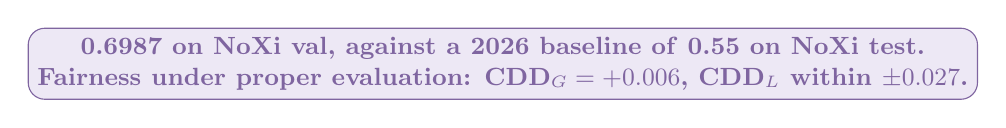
\begin{tikzpicture}
				\node[draw=coolpurple, fill=lightpurple, rounded corners=6pt,
				minimum width=11cm, minimum height=0.9cm, align=center,
				font=\small\bfseries, text=coolpurple] {
					\textbf{0.6987} on NoXi val, against a 2026 baseline of \textbf{0.55} on NoXi test.\\
					Fairness under proper evaluation: $\text{CDD}_G = +0.006$, $\text{CDD}_L$ within $\pm0.027$.
				};
			\end{tikzpicture}
		\end{center}
	\end{frame}

	% ============================== PART 4: SINCE AUGUST ==============================

	\begin{frame}{\textsc{Part 4:} Since August - Did We Keep The Right Checkpoint?}
		\begin{columns}[onlytextwidth]
			\begin{column}{0.44\textwidth}
				\begin{block}{Run 3, all saved checkpoints}
					\small
					\begin{tabular}{lr}
						Epoch & NoXi val CCC \\
						\hline
						10 & 0.6732 \\
						\textbf{16 (kept)} & \hl{0.6987} \\
						20 & 0.6267 \\
						30 & 0.6472 \\
					\end{tabular}
					\vspace{0.3em}

					\footnotesize \texttt{evaluate.py}, overlap-add. Only every 10th epoch was saved.
				\end{block}
			\end{column}
			\begin{column}{0.52\textwidth}
				\begin{block}{What this answers}
					\small
					\begin{itemize}
						\item The optimistic metric still picked the right one: of the four we
						have, epoch 16 is best.
						\item After epoch 16 the model gets \emph{worse}. ``Train longer so $\tau$
						fully anneals'' moves down the list.
						\item Checkpoints a few epochs apart differ by up to $0.07$. Any change
						smaller than that needs repeated runs before we believe it.
					\end{itemize}
				\end{block}
			\end{column}
		\end{columns}
	\end{frame}

	\begin{frame}{A Model Trained On One Corpus Is Nearly Blind On The Other}
		\begin{block}{Every model, scored on every corpus}
			\small
			\centering
			\begin{tabular}{lrr}
				& \textbf{Scored on NoXi} & \textbf{Scored on NoXi+J} \\
				\hline
				Trained on NoXi (Run 3) & \hl{0.6987} & 0.0922 \\
				Trained on NoXi+J (Run 1) & 0.1429 & \hl{0.4337} \\
			\end{tabular}

			\footnotesize NoXi: English, French, German. NoXi+J: Japanese, Chinese. Same features,
			same architecture, same task.
		\end{block}
		\begin{columns}[onlytextwidth]
			\begin{column}{0.48\textwidth}
				\begin{alertblock}{The off-diagonal is near zero}
					\small
					What a model learns about engagement on one set of people and languages
					barely transfers to the other.

					This is exactly the gap test-time adaptation was designed to close.
				\end{alertblock}
			\end{column}
			\begin{column}{0.48\textwidth}
				\begin{block}{Immediate consequence}
					\small
					Use one model per corpus. Mean over the two corpora goes
					from $0.3955$ to \hl{0.5662}.
					\vspace{0.2em}

					No new training, just the right model on the right data.
				\end{block}
			\end{column}
		\end{columns}
		\vspace{0.1em}
		\centering\footnotesize
		Side note: on NoXi+J the honest score (0.4337) is \emph{higher} than the training
		loop's (0.4228). The overlap-add gap is not a fixed discount.
	\end{frame}

	\begin{frame}{TTA - How It Is Supposed To Work}
		\begin{block}{The idea}
			\small
			At test time there are no labels. But the model has a \hl{fused} head that sees all
			8 streams, and 8 \hl{single-stream} heads that each see one. The fused head acts as a
			\emph{teacher}: on unlabelled test windows, we nudge the model so the single-stream
			heads agree with it.
		\end{block}
		\begin{block}{Only where teaching is safe and useful}
			\small
			Every head reports its uncertainty $u$ (the Beta variance from Part 0). Teach on
			window $i$ only if
			\begin{itemize}
				\item the teacher is \textbf{sure}: its $u$ is among the \emph{lowest} 30\% in the batch, and
				\item the students are \textbf{unsure}: their average $u$ is among the \emph{highest} 30\%.
			\end{itemize}
			Written out, with $q_p :=$ the value that a fraction $p$ of the batch falls below:
			$$ \text{keep}_i = \bigl[\,u^{\text{multi}}_i < q_{0.3}(u^{\text{multi}})\,\bigr]
			\;\wedge\; \bigl[\,u^{\text{uni}}_i > q_{0.7}(u^{\text{uni}})\,\bigr] $$
		\end{block}
	\end{frame}

	\begin{frame}{TTA Was Written, Wired In - And Never Fired}
		\begin{block}{With a batch of 10 windows}
			\small
			$q_{0.3}$ sits around the 3rd-lowest teacher uncertainty, so roughly the 3 surest windows
			pass the first test; $q_{0.7}$ sits around the 7th, so roughly the 3 most confused pass
			the second. Windows in both groups are kept.
		\end{block}
		\begin{alertblock}{Our inference feeds one window at a time}
			\small
			A batch of one. The 30\% point of a single number is that number,
			$q_{0.3}(\{u\}) = u$, and $u < u$ is never true.
			\hl{Every window is rejected, so the adaptation step is never called.}
		\end{alertblock}
		\begin{columns}[onlytextwidth]
			\begin{column}{0.48\textwidth}
				\begin{alertblock}{Two more problems behind it}
					\small
					Even when triggered, it adapts on \emph{every} window in the batch, not only
					the kept ones; and it outputs predictions from \emph{before} the update.
				\end{alertblock}
			\end{column}
			\begin{column}{0.48\textwidth}
				\begin{block}{What it means for our numbers}
					\small
					Every CCC in this talk is \textbf{without} TTA. The method in our paper's
					title has, in effect, never run - and the previous slides say we need it.
				\end{block}
			\end{column}
		\end{columns}
	\end{frame}

	\begin{frame}{What We Fixed}
		\begin{columns}[onlytextwidth]
			\begin{column}{0.48\textwidth}
				\begin{block}{In the model}
					\small
					\begin{itemize}
						\item Memory span: 58 ms $\to$ up to 40 s \hfill (P1)
						\item Modalities now actually fuse, the ordering matters,
						7.2M $\to$ 2.1M parameters \hfill (P2)
						\item One prediction per person, as the challenge asks \hfill (P3)
						\item Loss: ranking, hard frames, balance, fairness \hfill (P4)
					\end{itemize}
				\end{block}
			\end{column}
			\begin{column}{0.48\textwidth}
				\begin{block}{In the pipeline}
					\small
					\begin{itemize}
						\item Broken \texttt{NaN} entries in NoXi label files repaired
						\item Scoring through the real challenge pipeline, not the training loop
						\item Checkpoint choice re-checked on the real scores
						\item Found why TTA never fired
					\end{itemize}
				\end{block}
			\end{column}
		\end{columns}
		\vspace{0.6em}
		\begin{center}
			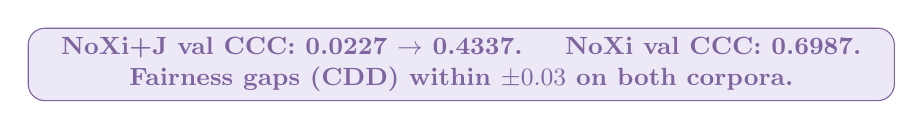
\begin{tikzpicture}
				\node[draw=coolpurple, fill=lightpurple, rounded corners=6pt,
				minimum width=11cm, minimum height=0.9cm, align=center,
				font=\small\bfseries, text=coolpurple] {
					NoXi+J val CCC: \textbf{0.0227} $\to$ \textbf{0.4337}. \quad NoXi val CCC: \textbf{0.6987}.\\
					Fairness gaps (CDD) within $\pm0.03$ on both corpora.
				};
			\end{tikzpicture}
		\end{center}
	\end{frame}

	\begin{frame}{Next Steps}
		\begin{block}{In order}
			\small
			\begin{enumerate}
				\item \textbf{Make TTA work, then run NoXi $\to$ NoXi+J} - it is the method in the
				title, and cross-corpus transfer ($0.09$) is exactly its job.
				\item \textbf{Submit per-corpus test predictions} - both models' test outputs are
				written, not yet checked.
				\item \textbf{Retrain NoXi+J with Run 3 settings} - running now; it was trained with
				older settings.
				\item \textbf{One model on both corpora} - does more data beat two specialists?
				\item \textbf{Repeat runs with different seeds} - checkpoints differ by up to $0.07$,
				so we need to know how much of any gain is noise.
				\item \textbf{Ablate the four loss terms} - which of them actually earns its place?
			\end{enumerate}
		\end{block}
		\vspace{0.4em}
		\centering\small
		Leaderboard context: best NoXi (base) test is $0.82$; the 2026 baseline is $0.55$.
	\end{frame}

\end{document}
